\documentclass{article}
\usepackage[landscape, margin=0.3in, top=0.5in, headheight=28pt, headsep=4pt]{geometry}
\usepackage{multicol}
\usepackage{tikz} 
\usetikzlibrary{decorations.pathmorphing}
\usetikzlibrary{fit}
\usepackage{xcolor}
\usepackage{fancyhdr}
\usepackage{enumitem}
\usepackage{fontspec}
\usepackage{titlesec}
\usepackage{amsmath}
\usepackage{graphicx}
\usepackage{svg}
\usepackage{float}
\usepackage{ifthen}
\usepackage{multirow}
\usepackage{colortbl}
\usepackage{caption}


\setmainfont[BoldFont={Montserrat-Medium}]{Montserrat-Regular}
\renewcommand{\baselinestretch}{0.9}
\renewcommand{\normalsize}{\fontsize{8}{8}\selectfont}

% Ensure the header/footer applies throughout
\thispagestyle{fancy}

% TikZ styles
\tikzstyle{mybox} = [draw=black, fill=white, very thick,
    rectangle, rounded corners, inner sep=4pt, inner ysep=4pt, minimum height=1cm, text centered, anchor=south]

\tikzstyle{fancytitle} = [
    draw=black,
    fill=black,
    very thick,
    rectangle, 
    rounded corners, 
    inner sep=4pt, 
    font=\bfseries\fontsize{10}{20}\selectfont\color{white}
]

\tikzstyle{fancytitleNull} = [draw opacity=0, fill opacity=0, very thick, rectangle, rounded corners, inner sep=4pt, font=\bfseries\fontsize{10}{20}\selectfont]

% Command definition for reusable fancybox
\newcommand{\fancybox}[2]{%
    \begin{tikzpicture}
        \node [mybox] (box) {%
            \begin{minipage}{0.9\linewidth} % Consistent width
            \vspace{8pt}
            #2
            \end{minipage}
        };
        
               \ifthenelse{\equal{#1}{}}{%
            % If title is empty
            \node[fancytitleNull, right=10pt] at (box.north west) {NULL};
        }{%
            % If title is not empty
            \node[fancytitle, right=10pt] at (box.north west) {#1};
        }      
    \end{tikzpicture}%
}

% Global adjustments for section headings
\titleformat{\section}[hang]{\small\bfseries}{\thesection}{1em}{}
\titlespacing*{\section}{0pt}{-3pt}{0.5pt}

% Global adjustments for subsection headings
\titleformat{\subsection}[hang]{\small\bfseries}{\thesubsection}{1em}{}
\titlespacing*{\subsection}{0pt}{-3pt}{0.5pt}

% Global adjustments for itemize lists
\let\olditemize\itemize
\def\itemize{\olditemize
  \renewcommand{\labelitemi}{\fontsize{8}{16}\selectfont$\bullet$}
}
\setlist[itemize]{left=6pt, itemsep=3pt, parsep=0pt, partopsep=0pt}
\setlist[enumerate]{left=6pt, itemsep=3pt, parsep=0pt, partopsep=0pt}

% Header settings
\pagestyle{fancy} % Enable fancy header and footer
\fancyhf{} % Clear default header and footer
\chead{\fontsize{14}{18}\selectfont \textbf{ISTQB - Certified Tester Foundation Level (CTFL) v4.0}}
\renewcommand{\headrulewidth}{0pt}
\rhead{\thepage}


% Footer customization
\cfoot{\textbf{Antonia Frey} \ \textperiodcentered\  \the\day-\the\month-\the\year} 
\renewcommand{\footrulewidth}{0pt} 
\setlength{\footskip}{0in} 




\begin{document}

\noindent
\begin{multicols}{3}

%------------ 1. Fundamentals of Testing ---------------
\fancybox{1. Fundamentals of Testing}{

\section*{What is Testing?}
Software testing is a set of activities to discover defects and evaluate the quality of software work products.

\section*{Why is Testing Necessary?}
Testing, as a form of quality control, helps in achieving the agreed upon test objectives within the set scope, time, quality, and budget constraints.\\

\section*{Testing and Debugging}
\begin{itemize}
\item \textbf{Testing} can trigger failures that are caused by defects in the software (dynamic testing) or can directly find defects in the test object (static testing)
\item \textbf{Debugging} is concerned with finding causes of this failure (defects), analyzing and eliminating them. 
\end{itemize}

\section*{Testing and Quality Assurance}
Testing is performed as a part of QC.
\begin{itemize}
  \item Testing is product-oriented
  \item QA is process-oriented
\end{itemize}

\section*{Errors, Defects, Failues, and Root Causes}
Human beings make errors (mistakes), which produce defects (faults, bugs), which may result in failures. Failures can also be caused by environmental conditions.\\

\section*{Testing Principles}
\begin{enumerate}
  \item Testing shows the presence of defects. 
  \item Exhaustive testing is impossible. 
  \item Early testing saves time and money. 
  \item Defects cluster together.
  \item Tests wear out.
  \item Testing is context dependent. 
  \item Absence-of-defects fallacy.
\end{enumerate}

\section*{Test Activities and Tasks}
\begin{itemize}
  \item Test planning
  \item Test monitoring and test control
  \item Test analysis
  \item Test design
  \item Test implementation
  \item Test execution
  \item Test completion
\end{itemize}

\section*{Roles in Testing}
\begin{itemize}
  \item \textbf{Test Management Role:} Takes overall responsibility for the test process, test team and leadership of the test activities.
  \item \textbf{Testing Role:} Focused on the activities of test analysis, test design, test implementation and execution.
\end{itemize}

\section*{Good Practices}
\begin{itemize}
    \item \textbf{Whole Team Approach:}
    Any team member can perform any task, everyone is responsible for quality.
    
    \item \textbf{Independence of Testing:}
    Independent testers recognize different kinds of failures and defects, but may be isolated from the development team, causing poor collaboration.
\end{itemize}
}

%------------ 2. Testing Throughout the SDLC ---------------
\fancybox{2. Testing Throughout the SDLC}{
\section*{Software Development Lifecycle (SDLC)}
An SDLC model is an abstract, high-level representation of the software development process. Every software development activity has a corresponding test activity.\\


\section*{Testing as a Driver for Software Development}
\begin{itemize}
  \item \textbf{Test-Driven Development (TDD)}\\
  Tests are written first, then the code is written to satisfy the tests.
  \item \textbf{Acceptance Test-Driven Development (ATDD)}\\
  Tests are derived from acceptance criteria and written before development of the application part. 
  \item \textbf{Behavior-Driven Development (BDD)}\\
  Tests are written in simple natural language (e.g., Given/When/Then) to express desired behavior.
\end{itemize}

\section*{Shift Left}
Approach where testing is performed earlier.\\

\section*{Test Levels}
Test levels are groups of test activities that are organized and managed together. There are five test levels:
\begin{itemize}
  \item \textbf{Component testing (unit testing)}\\
  Testing components in isolation.
  
  \item \textbf{Component integration testing}\\
  Testing interactions between components.
  
  \item \textbf{System testing}\\
  Testing the overall behavior and capabilities of an entire system or product, including functional and non-functional testing.
  
  \item \textbf{System integration testing}\\
  Testing interfaces of the system under test and other systems and external services.
  
  \item \textbf{Acceptance testing}\\
  Focuses on validation and on demonstrating readiness for deployment, which means that the system fulfills the user’s business needs.
\end{itemize}

\section*{Test Types}
\begin{itemize}
  \item \textbf{Functional testing} evaluates the functions that a component or system should perform. The functions are “what” the test object should do.
  \item \textbf{Non-functional testing} is the testing of “how well the system behaves”. These include aspects such as performance efficiency, compatibility, and usability.
  \item \textbf{Black-box testing} is specification-based.
  \item \textbf{White-box testing} is structure-based.
\end{itemize}

\section*{Confirmation Testing and Regression Testing}
\begin{itemize}
  \item \textbf{Confirmation Testing} confirms that an original defect has been fixed.
  \item \textbf{Regression Testing} confirms that no adverse consequences have been caused by a change.
\end{itemize}

\section*{Maintenance Testing}
The triggers for maintenance testing:\\
Modifications, Upgrades (Migrations), Retirement
}

%------------ 3. Static Testing ---------------
\fancybox{3. Static Testing}{
\section*{Static Testing Basics}
In contrast to dynamic testing, in static testing the software under test does not need to be executed. Static analysis can identify problems prior to dynamic testing while often requiring less effort, since no test cases are required, and tools are typically used.\\

\section*{Static Testing vs. Dynamic Testing}
\begin{itemize}
\item Some defect types that can only be found by either static or dynamic testing.
\item Static testing finds defects directly, while dynamic testing causes failures.
\item Static testing may more easily detect defects that lay on paths through the code that are rarely executed.
\item Static testing can be applied to non-executable work products.
\end{itemize}

\section*{Stakeholder Feedback}
Early and frequent feedback allows for the early communication of potential quality problems.\\

\section*{Review Process Activities}
\begin{itemize}
    \item Planning
    \item Review Initiation
    \item Individual Review
    \item Communication and Analysis
    \item Fixing and Reporting
\end{itemize}
\section*{Roles and Responsibilities in Reviews}
\begin{itemize}
    \item Manager – decides what to review and provides resources
    \item Author – creates and fixes the work product
    \item Moderator (also known as the facilitator) – runs review meetings and ensures a safe environment
    \item Scribe (also known as recorder) – records anomalies and decisions during the review
    \item Reviewer – performs the review, may be a subject expert or stakeholder
    \item Review leader – takes overall responsibility for review
\end{itemize}

\section*{Review Types}
\begin{itemize}
    \item Informal review – does not follow a defined process and does not require formal documented output.
    \item Walkthrough – led by the author, used for evaluating quality, building confidence, educating reviewers, and detecting anomalies.
    \item Technical Review – performed by technically qualified reviewers, led by a moderator. The goal is to make decisions regarding technical problems and detect anomalies.
    \item Inspection – the most formal type of review, following the complete generic process. The main objective is to find the maximum number of anomalies, evaluate quality, and improve the SDLC.
\end{itemize}
}

%------------ 4. Test Analysis and Design ---------------
\fancybox{4. Test Analysis and Design}{

\section*{Test Techniques}
\begin{itemize}

\item \textbf{Black-box Test Techniques (specification-based)}\\
Analysis of the specified behavior of the test object without reference to its internal structure. Therefore, the test cases are independent of how the software is implemented.

\begin{itemize}
    \item Equivalence Partitioning
    \item Boundary Value Analysis
    \item Decision Table Testing
    \item State Transition Testing
\end{itemize}

\item \textbf{White-box Test Techniques (structure-based)}\\
Analysis of the test object’s internal structure and processing. As the test cases are dependent on how the software is designed, they can only be created after the design or implementation of the test object.

\begin{itemize}
    \item Statement testing
    \item Branch testing
\end{itemize}

\item \textbf{Experience-based Test Techniques}\\
Use the knowledge and experience of testers for the design and implementation of test cases. These test techniques depends on the tester’s skills.

\begin{itemize}
    \item Error guessing
    \item Exploratory testing
    \item Checklist-based testing
\end{itemize}

\end{itemize}

\section*{Collaborative User Story Writing}
A user story represents a feature that will be valuable to either a user or purchaser of a system or software. User stories have three critical aspects, called the “3 C’s”:

\begin{itemize}
    \item \textbf{Card} – the medium describing a user story (e.g., an index card, an entry in an electronic board)
    \item \textbf{Conversation} – explains how the software will be used (can be documented or verbal)
    \item \textbf{Confirmation} – the acceptance criteria
\end{itemize}
The most common format for a user story is “As a [role], I want [goal to be accomplished], so that I can [resulting business value for the role]”, followed by the acceptance criteria.\\

\section*{Acceptance Criteria}
Acceptance criteria for a user story are the conditions that an implementation of the user story must meet to be accepted by stakeholders.\\

\section*{Acceptance Test-driven Development}
ATDD is a test-first approach. Test cases are created prior to implementing the user story. The test cases are based on the acceptance criteria and can be seen as examples of how the software works. Examples and tests are the same.
}

%------------ 5. Managing the Test Activities ---------------
\fancybox{5. Managing the Test Activities (1)}{
\section*{Test Plan}
A test plan describes the test objectives, resources and processes for a test project.\\

\section*{Entry Criteria and Exit Criteria}
Entry criteria define the preconditions for undertaking a given activity. Exit criteria define what must be achieved to declare an activity completed. Entry criteria and exit criteria should be defined for each test level, and will differ based on the test objectives.\\

\section*{Estimation Techniques}
\begin{itemize}
    \item \textbf{Estimation Based on Ratios}
    \item \textbf{Extrapolation}
    \item \textbf{Wideband Delphi} (e.g. Planning Poker)
     \begin{itemize}
        \item Commonly used in Agile SW development 
    \end{itemize}
    \item \textbf{Three-Point Estimation}\\
\vspace{-20pt}  
\begin{figure}[H]
  \begin{minipage}{0.5\textwidth}
  \text{Estimate:}\\
    \begin{equation*}
      E = \frac{a + 4m + b}{6} \quad \text{where:}
    \end{equation*}
    
  \end{minipage}
  \begin{minipage}{0.3\textwidth}
    \begin{flalign*}
      a & = \text{optimistic estimate} \\
      m & = \text{most likely estimate} \\
      b & = \text{pessimistic estimate}
    \end{flalign*}
  \end{minipage}
\end{figure}

\vspace{-20pt}  
\begin{figure}[H]
  \begin{minipage}{0.3\textwidth}
  \text{Measurement error:}\\
\begin{equation*}
SD = \frac{b - a}{6}
\end{equation*}
    
  \end{minipage}
  \begin{minipage}{0.7\textwidth}
  \end{minipage}
\end{figure}
 
\end{itemize}

\section*{Test Case Prioritization}
When prioritizing test cases, different factors can be taken into account. The most commonly used test case prioritization strategies are as follows:
\begin{itemize}
    \item \textbf{Risk-based prioritization}\\
    Test cases covering the most important risks are executed first.
    
    \item \textbf{Coverage-based prioritization}\\
    Test cases achieving the highest coverage are executed first.
    
    \item \textbf{Requirements-based prioritization}\\
    Test cases related to the most important requirements are executed first.
\end{itemize}

\section*{Test Pyramid}
 Tests in the bottom layer are small, isolated, fast, and check small pieces of functionality, a lot of them are needed for coverage. The top layer represents complex, high-level, end-to-end tests.
\begin{figure}[H]
  \begin{minipage}{0.45\textwidth}
    \centering
    \includesvg[width=\textwidth]{pyramid.svg}
  \end{minipage}%
  \hspace{0.05\textwidth} % Adjust space between image and text
  \begin{minipage}{0.5\textwidth}
  \raggedright % Left align the content
\begin{itemize}
\item UI tests,\\ end-to-end (E2E) tests 
\item Service tests,\\ Integration test
\item Unit tests,\\ Component tests
\end{itemize}
  \end{minipage}
\end{figure}

}

%------------ 5. Managing the Test Activities (2) ---------------
\fancybox{5. Managing the Test Activities (2)}{
\section*{Testing Quadrants}
The testing quadrants group the test levels with the appropriate test types, activities, test techniques and work products in the Agile software development.
\vspace{-10pt}
\begin{figure}[H]
    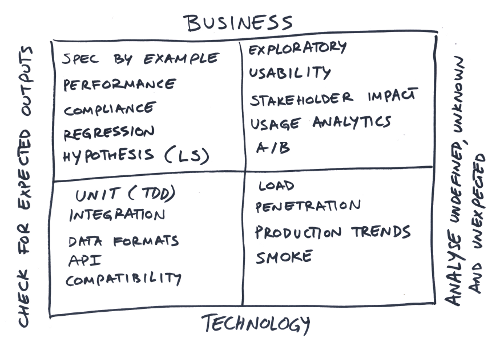
\includegraphics[width=0.8\textwidth]{quadrants.png}
    \vspace{-10pt}
\end{figure}


\begin{itemize}
  \item \textbf{Quadrant Q1} (technology facing, support the team): This quadrant contains component tests and component integration tests. These tests should be automated and included in the CI process.
  \item \textbf{Quadrant Q2} (business facing, support the team): This quadrant contains functional tests, examples, user story tests, user experience prototypes, API testing, and simulations. These tests check the acceptance criteria and can be manual or automated.
  \item \textbf{Quadrant Q3} (business facing, critique the product): This quadrant contains exploratory testing, usability testing, user acceptance testing. These tests are user-oriented and often manual.
  \item \textbf{Quadrant Q4} (technology facing, critique the product): This quadrant contains smoke tests and non-functional tests (except usability tests). These tests are often automated.
\end{itemize}

\section*{Risk Management}
The main risk management activities are:
\vspace{-5pt}
\begin{itemize}
  \item \textbf{Risk analysis}: Risk identification and -assessment
  \item \textbf{Risk control} Risk mitigation and -monitoring
\end{itemize}
A risk can be characterized by two factors:
\vspace{-5pt}
\begin{itemize}
\item Risk likelihood – probability of risk occurrence (0-1)
\item Risk impact (harm) – consequences of occurrence
\end{itemize}
In software testing there are two types of risks:
\vspace{-5pt}
\begin{itemize}
\item project risks - management issues
\item product risks - product quality characteristics
\end{itemize}

\section*{Product Risk Analysis}
Product risk analysis consists of \textbf{risk identification} and \textbf{risk assessment}. Risk assessment can use a quantitative or qualitative approach, or a mix of them.

\begin{itemize}
\item quantitative: $ \text{risk level} = \text{likelihood} * \text{impact}$
\item qualitative: risk level determined with risk matrix
\end{itemize}

}

%------------ 5. Managing the Test Activities (3) ---------------
\fancybox{5. Managing the Test Activities (3)}{

\section*{Monitoring, Control and Completion}
\begin{itemize}
\item \textbf{Test Monitoring}\\
Gathering information about testing.
\item \textbf{Test Control}\\
Uses the information from test monitoring to provide, in a form of the control directives, guidance and corrective actions to achieve better testing.
\item \textbf{Test Completion}\\
Collects data from completed test activities to consolidate experience, testware, and any other relevant information.
\end{itemize}

\section*{Metrics used in Testing}
\begin{itemize}
    \item Project progress metrics (e.g., task completion, resource usage, test effort).
    \item Test progress metrics (e.g., test case implementation progress, test environment preparation progress, number of test cases run/not run, passed/failed, test execution time).
    \item Product quality metrics (e.g., availability, response time, mean time to failure).
    \item Defect metrics (e.g., number and priorities of defects found/fixed, defect density, defect detection percentage).
    \item Risk metrics (e.g., residual risk level).
    \item Coverage metrics (e.g., requirements coverage, code coverage).
    \item Cost metrics (e.g., cost of testing, organizational cost of quality).
\end{itemize}

\section*{Configuration Management (CM)}
CM provides a discipline for identifying, controlling, and tracking work products such as test plans, test strategies, test conditions, test cases, test scripts, test results, test logs, and test reports as configuration items.\\

\section*{Defect Management}
Workflow for handling individual defects or anomalies from their discovery to their closure and rules for their classification.\\
}

%------------ 6. Test Tools ---------------
\fancybox{6. Test Tools}{
\section*{Tool Support for Testig}
\begin{itemize}
  \item \textbf{Test management tools}\\
  Tools to increase the test process efficiency by facilitating management of the SDLC, requirements, tests, defects, configuration
  
  \item \textbf{Static testing tools}\\
  Support tester in performing reviews and static analysis
  
  \item \textbf{Test design and test implementation tools}\\
  To generate test cases, data, and procedures
  
  \item \textbf{Test execution and test coverage tools}\\
  For automated test execution and coverage measurement
  
  \item \textbf{Non-functional testing tools}\\
  To perform non-functional testing that is difficult or impossible to perform manually
  
  \item \textbf{DevOps tools}\\
  Tools to support the DevOps delivery pipeline, workflow tracking, automated build processes, CI/CD
  
  \item \textbf{Collaboration tools} – facilitate communication
  \item \textbf{Tools supporting scalability and deployment standardization} (e.g., VMs, containerization tools)
\end{itemize}

\section*{Test Automation}
\textbf{Benefits of test automation:}
\begin{itemize}
  \item Provides \textbf{coverage measures} that are too complicated for humans to derive
  \item Time saved by reducing repetitive manual work
  \item Prevention of simple human errors
  \item More objective assessment
  \item Access to information (e.g., statistics, failure rates)
  \item Reduced test execution time
\end{itemize}

\textbf{Risks of test automation:}
\begin{itemize}
  \item Unrealistic expectations
  \item Inaccurate estimations of time, costs, effort
  \item Using a test tool when manual testing is more appropriate
  \item Relying on a tool too much
  \item Dependency on tool vendor
  \item Problems with open-source software
  \item Incompatiblility of tool with the development platform
  \item Unsuitable tool (Compliance and standards)
\end{itemize}
}

%------------ Test activities / Testware ---------------
\fancybox{Test activities / Testware}{
\begin{itemize}
    \item \textbf{Test planning:} Consists of defining the test objectives and then selecting an approach that best achieves the objectives within the constraints.
    
    \item \textbf{Test monitoring and control:}
Test monitoring involves the ongoing checking of all test activities and the comparison of actual progress against the plan. Test control involves taking the actions necessary to meet the objectives of testing.
    
    \item \textbf{Test analysis:} Includes analyzing the test basis to identify testable features and to define and prioritize associated test conditions (risk). The test basis and test objects are also evaluated to identify defects they may contain and to assess their testability. It is often supported by the use of test techniques and answers the question “what to test?”.
\begin{itemize}
\item \textbf{Testware:} 
prioritized test conditions (e.g., acceptance criteria), and defect reports for defects identified in the test basis
\end{itemize}    
    
    \item \textbf{Test design:} Includes elaborating the test conditions into test cases and other testware (e.g., test charters). This activity often involves the identification of coverage items, which serve as a guide to specify test case inputs. Test techniques can be used to support this activity. Test design also includes defining the test data requirements, designing the test environment, and identifying any other required infrastructure and tools. It answers the question “how to test?”.
\begin{itemize}
\item \textbf{Testware:}
prioritized test cases, test charters, coverage items, test data requirements, and test environment requirements
\end{itemize} 
    
    \item \textbf{Test implementation:} Includes creating or acquiring the testware necessary for test execution (e.g., test data). Test cases can be organized into test procedures and are often assembled into test suites. Manual and automated test scripts are created. Test procedures are prioritized and arranged within a test execution schedule for efficient test execution. The test environment is built and verified.
\begin{itemize}
\item \textbf{Testware:}
test procedures, automated test scripts, test suites, test data, test execution schedule, and test environment elements such as stubs, drivers, simulators, and service virtualizations
\end{itemize} 
    
    \item \textbf{Test execution:} Includes running the tests in accordance with the test execution schedule (test runs). Test execution may be manual or automated. Test execution can take many forms (continuous testing or pair testing sessions). Actual test results are compared with the expected results. The test results are logged. Anomalies are analyzed to identify their likely causes. This analysis allows us to report the anomalies based on the failures observed.
    
    \item \textbf{Test completion activities:} Occur at project milestones (e.g., release, end of iteration, test level completion) 
\begin{itemize}
\item \textbf{Testware:}
test completion report, documented lessons learned, action items for improvement, and change requests (as product backlog items)
\end{itemize}
\end{itemize} 
}

%------------ 4.2. Black-Box Test Techniques ---------------
\fancybox{4.2. Black-Box Test Techniques}{
\section*{Basics}
Black-box test technique, are based on an analysis of the specified behavior of the test object without reference to its internal structure. In black-box testing (specification-based) the test cases are based on an analysis of business logic, test cases are \textbf{not} based on the decisions in the source code. Therefore, test cases are independent of how the software is implemented.

\section*{1. Eqivalence Partitioning (EP)}
EP divides data into partitions. If a test case, that tests one value from an equivalence partition, detects a defect, this defect should also be detected by test cases that test any other value from the same partition. Therefore, one test for each partition is sufficient.\\

\section*{2. Boundary Value Analysis (BVA)}
BVA is a test technique based on exercising the boundaries of equivalence partitions. Therefore, BVA can only be used for ordered partitions. The minimum and maximum values of a partition are its boundary values. In the case of BVA, if two elements belong to the same partition, all elements between them must also belong to that partition.
\begin{itemize}
\item 2-value BVA
\item 3-value BVA
\end{itemize}

\section*{3. Decision Table Testing}
Decision tables are used for testing the implementation of requirements that specify how different combinations of conditions result in different outcomes. Decision tables are an effective way of recording complex logic, such as business rules.\\

\section*{4. State Transition Testing}
A state diagram models the behavior of a system by showing its possible states and valid state transitions. A transition is initiated by an event, which may be additionally qualified by a guard condition. The transitions are assumed to be instantaneous and may sometimes result in the software taking action. The common transition labeling syntax is as follows: “event [guard condition] / action”. Guard conditions and actions can be omitted if they do not exist or are irrelevant for the tester.
\begin{itemize}
\item \textbf{all states coverage}
\item \textbf{valid transition coverage}
\item \textbf{all transitions coverage}
\end{itemize}
All states coverage is weaker than valid transitions coverage, because it can typically be achieved without exercising all the transitions.\\

\subsection*{Which of the test activities are MOST likely to involve the application of BVA and EP?}
To identify the features that require testing, the test basis is analyzed and defined as test conditions, which are then prioritized along with related risks. The systematic identification of test conditions as coverage items often involves using \textbf{test techniques} both during \underline{test analysis} and as part of the \underline{test design} activity.
}

\fancybox{4.3. White-Box Test Techniques}{
\subsection*{Basics}
In white-box test techniques (structure-based testing), test cases are derived based on the source code structure. If a test case is based on the knowledge of the control flow of the test object, it is a white-box test technique. Test cases are based on an analysis of the test object’s internal structure and processing. As the test cases are dependent on how the software is designed and coded, they can only be created after the design or implementation of the test object.\\

\section*{Value of White-box Testing}
White-box test techniques can be used in static testing (e.g., during dry runs of code). They are well suited to reviewing code not yet ready for execution, pseudocode and other high-level or top-down logic which can be modeled with a control flow graph.\\

\section*{1. Statement Testing and Statement Coverage}
In statement testing, the coverage items are executable statements. The aim is to design test cases that exercise statements in the code until an acceptable level of coverage is achieved. Coverage is measured as the number of statements exercised by the test cases divided by the total number of executable statements in the code, and is expressed as a percentage.\\

\section*{2. Branch Testing and Branch Coverage}
In branch testing, the test cases are derived from knowledge of the control flow of the test object.\\
A branch is a transfer of control between two nodes in the control flow graph, which shows the possible sequences in which source code statements are executed in the test object. Each transfer of control can be either \textbf{unconditional} (i.e., straight-line code) or \textbf{conditional} (i.e., a decision outcome).\\

\subsection*{Branch coverage metric}
The formula for branch coverage $B_{\text{Cov}}$ is given by:
\begin{equation*}
    B_{\text{Cov}} = \left( \frac{\text{branches exercised by test cases}}{\text{total number of branches in code}} \right) \times 100\% 
    \end{equation*}

\subsection*{Branch coverage vs statement coverage}
Branch coverage subsumes statement coverage. This means that any set of test cases achieving 100\% branch coverage also achieves 100\% statement coverage (but not vice versa).\\

\subsection*{Statement coverage}
Test T1 achieved 40\% statement coverage and test T2 achieved 65\% statement coverage.\\
The statements executed by T1 and T2 were disjoint, the coverage of the test suite {T1, T2} would be 105\%, which is impossible. At least 5\% of executable statements must have been executed by both T1 and T2.
}

%------------ Anomalies ---------------
\fancybox{Anomalies}{
\section*{Def. "Anomalies"}
Deviations from expected behavior in software:\\
\begin{itemize}
\item (real) defects or bugs - errors in the code
\item failures - system does not perform as intended
\item errors - mistakes made by developers, ...
\item false-positives – non-issues flagged as problems
\item change request
\end{itemize}
}

%------------ 4.4. Experience-based Test Techniques ---------------
\fancybox{4.4. Experience-based Test Techniques}{
\section*{1. Error guessing}
Error guessing is a test technique used to anticipate the occurrence of errors, defects, and failures, based on the tester’s knowledge, including:
\begin{itemize}
\item How the application has worked in the past
\item The types of errors the developers tend to make and the types of defects that result from these errors
\item The types of failures that have occurred in other, similar applications
\end{itemize}

\section*{2. Exploratory testing}
In exploratory testing, tests are simultaneously designed, executed, and evaluated while the tester learns about the test object. The testing is used to learn more about the test object, to explore it more deeply with focused tests, and to create tests for untested areas.\\

Exploratory testing is most useful when there are few known specifications and/or there is a pressing timeline for testing (e.g., delay in the release of a brand-new application).\\

\section*{3. Checklist-based testing}
In checklist-based testing, a tester designs, implements, and executes tests to cover test conditions from a checklist. Checklists can be built based on experience, knowledge about what is important for the user, or an understanding of why and how software fails. Checklists should not contain items that can be checked automatically, items better suited as entry criteria, exit criteria, or items that are too general.
}

%------------ Acceptance Criteria ---------------
\fancybox{Acceptance Criteria}{
\section*{Basics}
Acceptance criteria are a set of predefined requirements or conditions that a product, feature, or functionality must meet to be considered complete and acceptable to stakeholders.\\

\section*{Format}
\begin{itemize}
\item \textbf{Scenario-Oriented Format (Given-When-Then)}\\
Given/When/Then is a scenario-oriented format because it describes a scenario to be verified.
\item \textbf{Rules-Based Format}\\
The rule-oriented format includes formats like bullet point verification lists or tabulated forms of input-output mappings, explicitly showing the rules to be followed. 
\end{itemize}
}

%------------ Validation vs Verification ---------------
\fancybox{Validation vs Verification}{
\begin{itemize}
\item \textbf{Validation} is concerned with meeting user requirements and expectations
\item \textbf{Verification} is concerned with meeting specified requirements
\end{itemize}

Acceptance testing focuses on validation and on demonstrating readiness for deployment, which means that the system fulfills the user’s business needs. Ideally, acceptance testing should be performed by the intended users. The main forms of acceptance testing are: user acceptance testing (UAT), operational acceptance testing, contractual and regulatory acceptance testing, alpha testing and beta testing.
}

%------------ Reviews ---------------
\fancybox{Reviews}{
\subsection*{Review activities}
\begin{itemize}
\item \textbf{Planning}\\
Defining the review scope, purpose, work product to be reviewed, quality characteristics to be evaluated, areas of focus, exit criteria, supporting information such as standards, effort, and timeframes.)

\item \textbf{Review initiation}\\
Ensuring all participants have access to the work product and necessary resources, and clarifying their roles and responsibilities.

\item \textbf{Individual review}\\
Evaluating the work product's quality, identifying and logging anomalies, recommendations, and questions using review techniques like checklist-based and scenario-based reviewing.

\item \textbf{Communication and analysis}\\
Analyzing and discussing each anomaly, determining its status, ownership, and required actions, and making review decisions, normally in a meeting. This could include determining the need for a follow-up review.

\end{itemize}


\subsection*{Roles in reviews}
\begin{itemize}
\item \textbf{Scribe (or Recorder)}\\
Responsible for gathering feedback and recording information from reviewers and documenting review information, such as decisions made, and any new anomalies identified during the review meeting.

\item \textbf{Review Leader}\\
Responsible for overseeing the review process, such as selecting the review team members, scheduling review meetings (organizing when and where), and ensuring that the review is completed successfully.

\item \textbf{Facilitator (or Moderator)}\\
Responsible for ensuring that the review meetings run effectively, including managing time, mediating discussions, and creating a safe environment where everyone can voice their opinions freely.

\item \textbf{Manager}\\
Responsible for deciding what needs to be reviewed and allocating resources, such as staff and time, for the review.
\end{itemize}
}


%------------ Metrics ---------------
\fancybox{Metrics}{
\begin{itemize}
\item \textbf{Product quality metrics}\\
Mean time to failure (measures maturity)
\item \textbf{Defect metric}\\
Number of defects found, Defect detection percentage 
\item \textbf{Coverage metric}\\
Requirements coverage
\end{itemize}
}




%------------ Keywords (K1) ---------------
\fancybox{Keywords (K1)}{
\section*{Overview}
All keywords shall be remembered (K1).\\

\section*{1. Fundamentals of Testing}
coverage, debugging, defect, error, failure, quality, quality assurance, root cause, test analysis, test basis, test case, test completion, test condition, test control, test data, test design, test execution, test implementation, test monitoring, test object, test objective, test planning, test procedure, test process, test result, testing, testware, traceability, validation, verification\\

\section*{2. Testing Throughout the SDLC}
acceptance testing, black-box testing, component integration testing, component testing, confirmation testing, functional testing, integration testing, maintenance testing, non-functional testing, regression testing, shift left, system integration testing, system testing, test level, test object, test type, white-box testing\\

\section*{3. Static Testing}
anomaly, dynamic testing, formal review, informal review, inspection, review, static analysis, static testing, technical review, walkthrough\\

\section*{4. Test Analysis and Design}
acceptance criteria, acceptance test-driven development, black-box test technique, boundary value analysis, branch coverage, checklist-based testing, collaboration-based test approach, coverage, coverage item, decision table testing, equivalence partitioning, error guessing, experience-based test technique, exploratory testing, state transition testing, statement coverage, test technique, white-box test technique\\

\section*{5. Managing the Test Activities}
defect management, defect report, entry criteria, exit criteria, product risk, project risk, risk, risk analysis, risk assessment, risk control, risk identification, risk level, risk management, risk mitigation, risk monitoring, risk-based testing, test approach, test completion report, test control, test monitoring, test plan, test planning, test progress report, test pyramid, test strategy, testing quadrants\\

\section*{6. Test Tools}
test automation
}

%------------ Certification ---------------
\fancybox{Certification}{

\section*{ISTQB}
The International Software Testing Qualifications Board (ISTQB) is a software testing certification board.\\

\section*{Overview}
The ISTQB Certified Tester Foundation Level (CTFL) certification is the cornerstone of essential testing knowledge that can be applied to real-world scenarios.\\

\section*{Exam Structure}
\begin{itemize}
    \item \textbf{No. of Questions}: 40
    \item \textbf{Passing Score}: 26
    \item \textbf{Total Points}: 40
    \item \textbf{Time (min)}: 60 (+15 min for Non-Native Language)
\end{itemize}

\section*{Learning objectives levels}
\begin{itemize}
\item K1: Remember
\item K2: Understand
\item K3: Apply
\end{itemize}

\vspace{10pt}
\section*{Exam Structures Rules}
\vspace{-10pt}
\begin{table}[H]
\renewcommand{\arraystretch}{1.8}
\centering
\begin{tabular}{|c|c|c|c|}
\hline
\rowcolor{black} \textcolor{white}{\textbf{K-Level}} & 
\textcolor{white}{\textbf{No. of Questions}} & 
\textcolor{white}{\textbf{Time}} & 
\textcolor{white}{\textbf{Total Time}} \\ \hline
K1                              & 8                                              & 1                                    & 8                       \\ \hline
K2                              & 24                                             & 1                                    & 24                      \\ \hline
K3                              & 8                                              & 3                                    & 24                      \\ \hline
\hline
\textbf{Total}                 & \textbf{40}                                    &                               & \textbf{56 min}             \\ \hline
\end{tabular}
\vspace{-5pt}
\caption*{K-Level Breakdown and Total Time}
\end{table}

\vspace{-15pt}
\begin{table}[H] 
\renewcommand{\arraystretch}{1.8}
\centering
\begin{tabular}{|c|c|c|c|c|c|}
\hline
\cellcolor{black}\textcolor{white}{\textbf{Chapter}} & \cellcolor{black}\textcolor{white}{\textbf{K1}} & \cellcolor{black}\textcolor{white}{\textbf{K2}} & \cellcolor{black}\textcolor{white}{\textbf{K3}} & \cellcolor{black}\textcolor{white}{\textbf{Points}} & \cellcolor{black}\textcolor{white}{\textbf{Percentage}} \\ \hline
\textbf{Chapter 1} & 2 & 6 & 0 & 8 & \textbf{13\%} \\ \hline
\textbf{Chapter 2} & 1 & 4 & 0 & 5 & \textbf{8\%} \\ \hline
\textbf{Chapter 3} & 1 & 3 & 1 & 5 & \textbf{8\%} \\ \hline
\textbf{Chapter 4} & 1 & 5 & 5 & 11 & \textbf{18\%} \\ \hline
\textbf{Chapter 5} & 2 & 5 & 2 & 9 & \textbf{15\%} \\ \hline
\textbf{Chapter 6} & 1 & 1 & 0 & 2 & \textbf{3\%} \\ \hline \hline
\textbf{Total} & 10 & 24 & 8 & 60 & 100\% \\ \hline
\end{tabular}
\vspace{-5pt}
\caption*{Question Breakdown by Chapter and K-Level}
\end{table}
}


\end{multicols}

\end{document}
